\chapter{Colour Spaces}
\label{ch:cs}

Colour spaces are a fundamental element in colour science. They establish the primary colours and the geometric representation of the range of colours that can be reproduced within a specific colour space. Additionally, they often include criteria for quantifying the differences between sets of colours. For instance, the colour matching functions depicted in Figure \ref{fig:xyz} constitute the CIE XYZ 1931 colour space, as defined by \cite{cie1931}.

Colour spaces can roughly be divided into two types: device-independent and device-dependent colour spaces. In the former, the colour values are not tied to any particular device. They are instead based on human visual perception or standardized models, while in the latter, the interpretation of specific colour values can vary wildly across devices.


\section{Device-independent colour spaces}

Device-independent colour spaces can be further divided into three subcategories: reference colour spaces, output-referred colour spaces and perceptually uniform colour spaces \cite[ch.~4.1-4.5]{rowlands2020physics}. The last two are always related to the first by some known transformation. 

Since colour values in device-independent colour spaces have universal meaning, they can also be easily visualized, and the set of reproducible colours can be compared. However as colour spaces are three-dimensional, and form complex shapes, one dimension is often dropped for visualization purposes, resulting in a so-called chromaticity diagram \cite[42-44]{measuringcolour}.

Three different colour spaces are shown on a chromaticity diagram in \ref{fig:gamut}. The filled horseshoe-shaped figure corresponds to the colours a human could theoretically see, while the two smaller triangles, in this case, Adobe Adobe RGB \cite{adobeRGB} and sRGB \cite{sRGB}, are subspaces of the former. The colours inside the outlined shapes form the gamut of a colour space, which contains the set of colours reproducible by the space or a system.

\begin{figure}
    \centering
    \pdftooltip{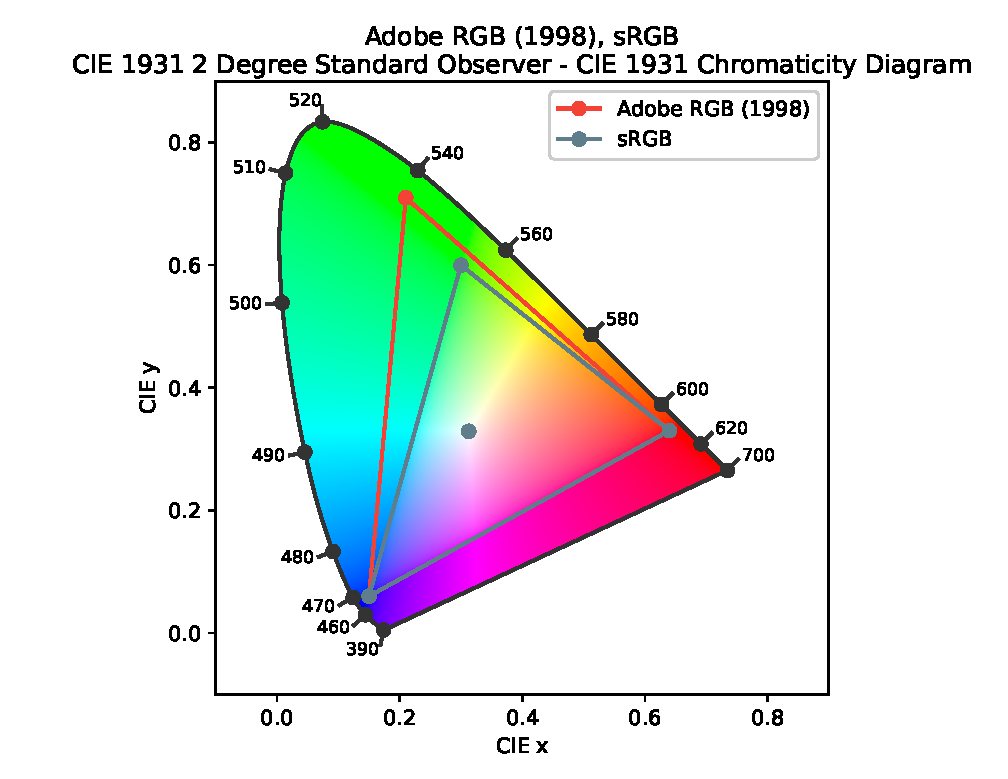
\includegraphics[width=\textwidth]{figures/gamut.eps}}{ Gamut}
    \caption{CIE XYZ \cite{cie1931}, Adobe RGB \cite{adobeRGB} and sRGB \cite{sRGB} colour gamuts on a chromaticity diagram}
    \label{fig:gamut}
\end{figure}


\subsection{Reference colour spaces}

Colour spaces which contain all colours in the visible range are known as reference colour spaces. These include 
for example the CIE XYZ colour space seen in figure \ref{fig: gamut}. Reference spaces allow us to move to other linearly related spaces by changing their basis, which makes them convenient. Furthermore, they are often used as target colour space when the input is in camera-specific colour space. \cite[224-225]{rowlands2020physics}


\subsection{Output-referred spaces}

Output-referred colour spaces define a standard for output devices, ensuring manufacturers interpret a set of colour values similarly. Otherwise, two manufacturers could use proprietary formats and thus an image would produce different colours on different devices. To this date, output-referred colour spaces occupy only a subset of the reference colour spaces, partially because an additive mixture of three primaries cannot represent all colours visible to humans \cite[65]{colorimetry}. The most common colour spaces, such as sRGB and Adobe RGB, are based on red, green and blue primaries and thus only a subset is reproducible as is visible in \ref{fig:gamut}.

\subsection{Uniform colour spaces}

It is often necessary to measure the difference between two colours, such as to compare how accurately an algorithm produces colours compared to how an observer would have seen them. However, even when using reference color spaces with a geometrical interpretation, it is not guaranteed that two pairs of colours with the same geometrical distance will appear equally different to an observer. To optimize algorithms for perceptual quality, it is important to create colour spaces that take this into account.

Uniform color spaces, although not perfect, attempt to ensure that colours with the same distance in the space correspond to being equally different to an observer.
